\chapter{Déroulement du projet}
\label{sec:deroulement}

\section{Prise en main du sujet et des technologies}
	Après avoir développé la partie sur les explications techniques, nous allons détailler le déroulement du projet pour notre binôme. Pour commencer, nous devions prendre en main les différents outils nécessaires au projet.
	
	\subsection{Contiki}
	Comme nous avons déjà vu, Contiki est un système d'exploitation  embarqué. Notre expérience avec le domaine de l'embarqué était limitée malgré notre curiosité, bien que Théo ait fait un stage en rapport pendant sa licence. Nous avons étudié les systèmes d'exploitation lors de cette année de master, mais pas les systèmes embarqués en particulier. L'interaction avec Contiki s'est fait assez rapidement, mais sa compréhension réelle s'est avérée cependant difficile.\\
	Certains concepts, comme les proto-threads (parallélisation très légère avec une taille mémoire limitée) utilisés par Contiki, sont assez proches d'autres concepts présents dans les systèmes d'exploitation habituels, néanmoins la découverte des autres fonctionnalités de Contiki s'est fait au fur et à mesure. En effet Contiki possède de nombreuses caractéristiques en plus de celles qu'offrent les systèmes embarqués habituels.\\
	Ces notions, en plus de celles déjà évoquées sur IPv6 et 6LoWPAN, nous confortent dans le choix de Contiki plutôt que FreeRTOS ou TinyOS, qui regroupe l'ensemble des caractéristiques des autres OS.
%		\begin{itemize}
%			\item Embarqué
%			\item simulations avec Cooja
%			\item Pourquoi Contiki et pas un autre ?
%		\end{itemize}

	\subsection{Chaîne de compilation et pilotes}
	L'utilisation des chaines de compilations s'est faite rapidement puisque la machine virtuelle InstantContiki3.0 en possède déjà une pour les projets existants et leur différente architecture supportée par Contiki. Les différents tutoriels présents sur le web ont facilités l'installation manuelle de ces chaînes de compilation.\\
	En revanche, les pilotes des différents contrôleurs radios nous ont semblé difficiles à prendre en main. Nous avons également choisi de nous concentrer sur les contrôleurs cc2420 ( utilisés pour les communications sans-fils ) de Texas Instrument puisqu'ils sont déjà présents dans les autres projets.
%		\begin{itemize}
%			\item GCC
%			\item architectures différentes
%			\item contrôleurs radio différents
%		\end{itemize}

\section{Programme développé}
	Le programme développé a été une mise en pratique de nos recherches, mais comme évoqué avant, la prise en main des technologies utilisées a été plutôt longue.
	\subsection{Fonctionnement du projet}
		La sonde renifleuse capture les paquets dans le trafic du réseau, en les récupérant à la couche radio de la pile réseau, donc récupère tous les paquets, y compris ceux qui ne sont pas conformés à 6LoWPAN.\\
		Les paquets sont triés et stockés dans les buffers cycliques pour permettre des vérifications plus en profondeur.\\
		Le triage se fait en interprétant l'en-tête bit par bit, en se basant sur les explications des RFC pour déterminer les différentes caractéristiques du paquet.
		\begin{figure}[htp]
			\centering
			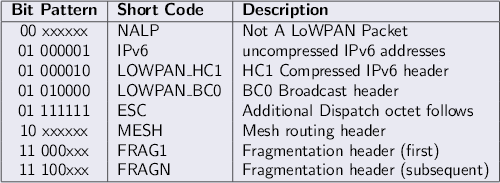
\includegraphics[width=15cm]{images/parsing}
			\caption{Exemple de tableau aidant à l'interprétation des paquets.}
			\label{fig:parsing}
		\end{figure}
	\subsection{État du projet}
		Ce projet a évolué au fur et à mesure de nos avancées, et bien que nous ayons défini des vérifications, nous n'avons pas pu implémenter tout ce que nous voulions.\\
		Le triage des paquets est encore à gros grains, et l'utilisation des buffers cycliques ne marche pas complètement. Certains bugs à la compilation nous empêche de les utiliser comme nous le voulons.\\
		Nous avions prévu d'implémenter des vérifications sur les tailles des paquets, la taille annoncée par rapport à la taille réelle, mais l'interprétation des en-têtes a été prioritaire car c'est elle qui nous permet d'accéder au champ en question.

\section{Retours d'expérience} % DONE ?
    Durant notre projet, nous avons eu l'opportunité d'améliorer nos compétences dans les différents domaines du web des objets. Ce travail pourra bénéficier d'évolutions sur le court comme sur le long terme.
    
	\subsection{Évolutions à court terme} % DONE
	Sur le court terme, il serait possible d'ajouter d'autres types de détections d'attaques en fonction des besoins, mais ces ajouts ne sont pas pertinent dans le cadre de notre projet. En effet l'équipe de recherche 2XS souhaite intégrer la sonde dans Discus qui est déjà un système de détection d'intrusion, ce qui rendrait ces modifications redondantes.\\
	La sonde pourrait donc fournir les informations dont Discus a besoin pour faire respecter les contraintes énoncée dans le script adéquat.\\ 
	De ce fait, les vérifications d'attaques seraient donc effectuées par le système qui reçoit les informations, et non plus par les sondes directement. Ceci permet d'alléger la charge de travail sur les capteurs aux capacités restreintes. Aussi, les nouvelles vérifications d'intrusion pourront êtres implémentées sans reprogrammer les sondes.
	\subsection{Évolutions à long terme} % DONE
	Sur un plus long terme, il a été pensé d'éventuellement faire communiquer les sondes entre elles afin de créer une grille de capteurs.
	Cela permettrait, grâce aux différents RSSI associés à un seul paquet capté, de localiser les différents acteurs du réseau, et donc de localiser l'attaquant lors d'une anomalie.
	\subsection{Challenges} % DONE
	 Ce projet a été enrichissant et concernait les domaines qui nous intéressent (comme l'embarqué et/ou la sécurité), mais nous avons dû faire face à plusieurs difficultés et challenges lors de son déroulement. Bien que ces contraintes ralentissaient l'avancement du projet, elles furent instructives à plusieurs niveaux.\\
	 Tout d'abord, le sujet se concentre sur des domaines et technologies dont nous n'étions pas très familiers. Le monde de l'informatique embarquée est fait de contraintes auxquelles il faut s'adapter pour être productif, les retours beaucoup moins verbeux lors d'erreurs, les limites de mémoire, de puissance, et parfois l'absence de librairies pour rendre le code assez léger pour la plateforme sont quelques exemples de difficultés lorsque l'on découvre l'embarqué. Pouvoir s'adapter peut paraître laborieux mais la solution est de bien organiser le contexte et prendre le temps nécessaire pour assimiler les bases.\\
	 Les découvertes étaient nettement plus nombreuses dans les technologies employées, notamment au niveau des systèmes d'exploitation embarqués, comme Contiki, et leurs technologies de communication. Nous avons lu beaucoup de spécifications, de RFC et de documentation et en rétrospective, nous aurions eu plus de facilité à établir un plan d'approche, organiser nos découvertes pour éviter la confusion. Par exemple, prendre du temps pour bien se renseigner sur Contiki, puis lorsque l'outil est maîtrisé, se renseigner sur 6LoWPAN, et continuer à procéder par étapes durant l'ensemble du pji.\\
	 Malgré nos recherches en profondeur, nous sommes parfois tombés sur des incohérences dans la documentation, ou des explications confuses, notamment sur le buffer de paquets qui n'a pas la même structure si les paquets sont entrants ou sortants. Pour pallier à ce souci, nous nous sommes documentés sur des sites et des encyclopédies en ligne (wikis) universitaires traitant de Contiki avec des tutoriels adaptés à notre besoin.\\
	 Une autre difficulté durant le projet venait de Contiki lui même. En effet, certains exemples de code déjà présents ne sont pas assez commentés, ceci peut être problématique pour assimiler le fonctionnement d'un programme. C'est pourquoi nous nous sommes rendus sur des forums traitant de ces sujets et avons sollicité des membres de l'équipe 2XS.

%%% Local Variables: 
%%% mode: latex
%%% TeX-master: "isae-report-template"
%%% End: 
